\documentclass[11pt]{article}

\usepackage{comment} % enables the use of multi-line comments (\ifx \fi) 
\usepackage[a4paper,margin=1cm]{geometry}
\usepackage[utf8]{inputenc}
\usepackage[ngerman]{isodate}
\usepackage{gensymb}
\usepackage{graphicx}
\usepackage{booktabs}% http://ctan.org/pkg/booktabs
\usepackage{tabularx}
\usepackage{ltablex} % Longtables with tabularx
\usepackage[x11names]{xcolor}
\usepackage{amsmath}
\usepackage{amssymb}
\usepackage{amsthm}
\usepackage{array}
\usepackage{wrapfig}
\usepackage{subcaption}
\usepackage{csquotes}
\usepackage{lscape}
\usepackage{geometry}
\usepackage{multicol}
\usepackage{bm}
\usepackage{enumitem}
\usepackage{hyperref}
\usepackage{mdframed}
\usepackage{scalerel}
\usepackage{stackengine}
\usepackage{mathtools}
\usepackage{pdfpages}

% Code highlighting
\usepackage{minted}
\surroundwithmdframed{minted}

% Be able to caption equations and float them in place
\usepackage{float}

\newmdtheoremenv{theorem}{Theorem}

\theoremstyle{definition}
\newmdtheoremenv{definition}{Definition}[section]


\geometry{a4paper, margin=2.4cm}

\newcommand\equalhat{\mathrel{\stackon[1.5pt]{=}{\stretchto{\scalerel*[\widthof{=}]{\wedge}{\rule{1ex}{3ex}}}{0.5ex}}}}
\newcommand\defeq{\mathrel{\overset{\makebox[0pt]{\mbox{\normalfont\tiny def}}}{=}}}
\newcolumntype{C}{>{\centering\arraybackslash}X}

\DeclarePairedDelimiter\abs{\lvert}{\rvert}
\DeclarePairedDelimiter\norm{\lVert}{\rVert}

\newcommand*\samplemean[1]{\overline{#1}}
\newcommand*\ev[1]{\mathrel{\text{E}\left[#1\right]}}
\newcommand*\R{\mathbb{R}}
\newcommand*\Z{\mathbb{Z}}
\newcommand*\diff{\mathop{}\!\mathrm{d}}
\newcommand*\Diff[1]{\mathop{}\!\mathrm{d^#1}}
\newcommand*\Exp[1]{\mathop{\text{Exp}}\left(#1\right)}
\newcommand*\Cov[1]{\mathop{\text{Cov}}\left(#1\right)}
\newcommand*\Cor[1]{\mathop{\text{Cor}}\left(#1\right)}
\newcommand*\Var[1]{\mathop{\text{Var}}\left(#1\right)}

\setcounter{tocdepth}{3}
\setcounter{secnumdepth}{3}

\graphicspath{{./img/}}

\begin{document}
	
\title{Machine Learning FS20}
\author{Pascal Baumann\\pascal.baumann@stud.hslu.ch}
\maketitle



For errors or improvement raise an issue or make a pull request on the \href{https://github.com/KilnOfTheSecondFlame/mse_summaries}{github repository}.

\tableofcontents
\newpage



\section{Introduction}

\subsection{Inductive Learning}

Inductive learning has the goal to \textbf{discover general concepts} from a \textbf{limited set of examples}, a model using inductive reasoning obtains new general knowledge from specific information. Throughout the learning process it is not truth preserving, new information can invalidate the current model, and works heuristically. The assumption therefore is that a model fitted to a sufficiently large learning set will be able to generalise to unseen data.

\begin{landscape}
	\subsubsection{Machine Learning Flowchart}
	\begin{center}
		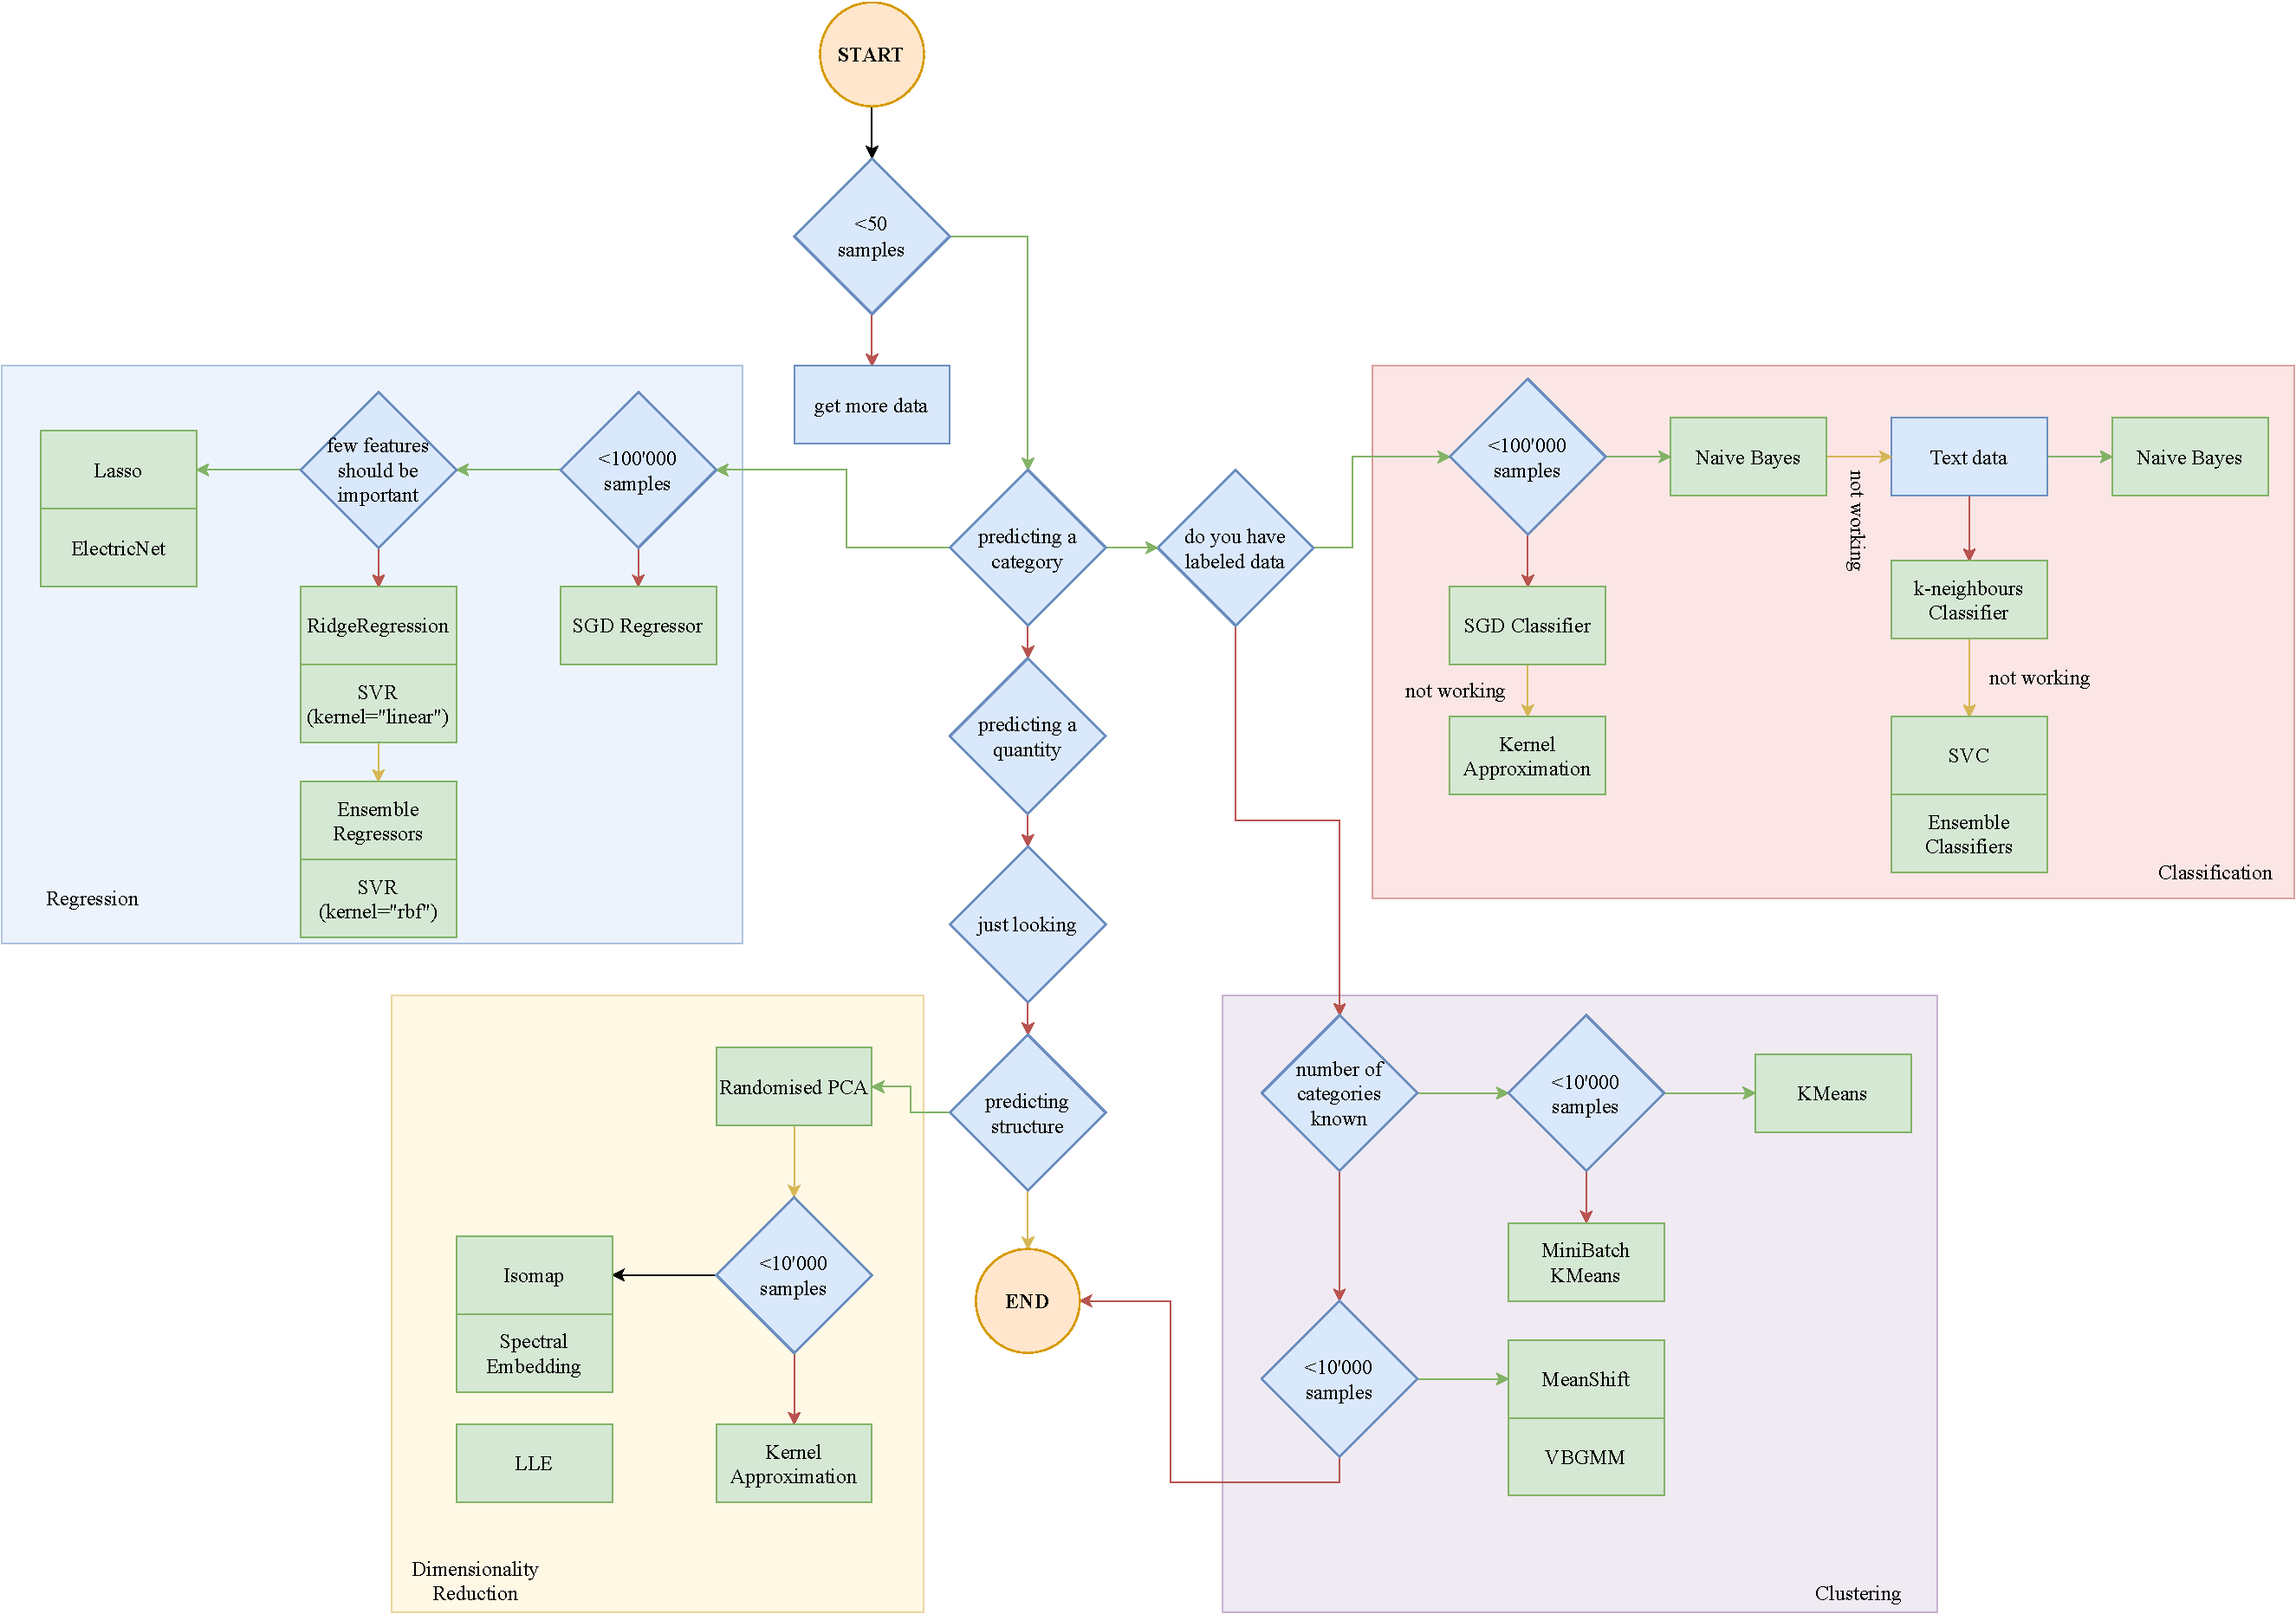
\includegraphics[height=0.9\textheight, keepaspectratio]{scikit-learn_algorithm_cheatsheet}
	\end{center}
\end{landscape}

\subsection{Inductive Supervised Learning}
The data usually has a semi-formal representation in attribute-label pairs $(\textbf{x}, y)$. The labels encode concepts or classes.
Approximate the mapping function from example $x$ to label $y$ with a hypothesis $h(x) = \hat{y} \approx f(x)$ so that it generalises well.

\subsection{Learning as Search}
\begin{center}
	\includegraphics[width=0.7\linewidth]{"../Machine Learning in Computer Visualisation/img/hypothesis_space"}
\end{center}

The hypothesis space $\mathcal{H}$ contains all possible hypotheses that can be built with the chosen representation, learning can thus be understood as a search for the global minima in this space $\mathcal{H}$.

\noindent
Formally this goal is expressed as follows: Find the hypothesis $h^* (x,\theta) = \hat{y}$ that best fits the training data, according to a loss function $L(h(x,\theta))$ by searching the hypothesis space $\mathcal{H} = \left\{ h(x,\theta) \middle| \theta \in P\right\}$.

\subsection{Inductive Bias}
\begin{theorem}
	A learner that makes \textbf{no a-priori assumptions} regarding the identity of the target concept has \textbf{no rational basis for classifying} any unseen instances. - Mitchell
\end{theorem}
All learning algorithms have some preformed hypothesis that is helpful to look for. It is beneficial to choose algorithms whose implicit hypothesis fits the data.

No free lunch theorem regarding the general equivalence of learners states that if all functions $f$ are equally likely, the probability of observing an arbitrary sequence of cost values during training does not depend on the learning algorithm $\mathcal{L}$.

The inductive bias of a learning algorithm $\mathcal{L}$ for instances in $X$ are any \textbf{minimal set of assertions} $B$ that, together with $\mathcal{L}$ and the training set $D$ \textbf{allows for deductively inferring} the $y'$ for a new $x\in X$. Make all assumptions \textbf{explicit} in $B$ such that $\forall x' \in X: \left(B, \mathcal{L}, D, x' \right) \Rightarrow y'$ is provable.

Machine Learning depends on the intelligent choice of the class $\mathcal{H}$ where $\mathcal{L}$ optimises the parameters. Machine Learning algorithms can be categorised by the strength of their inductive bias.

\subsection{Inductive Unsupervised Learning}
\begin{minipage}{0.6\linewidth}
	The usual task is Clustering, where the data $D$ are described by feature vectors without any labels, interesting structures and relationships in the data are then searched. The data naturally fall into $K$ groups, where the number of classes are not determined at the start but found through the learning scheme. This presents the challenge of searching by similarity in \textbf{distance} or \textbf{density}, which is another inductive bias to be considered, and by the choice of \textbf{parameters}.
	
\end{minipage}
\begin{minipage}{0.4\linewidth}
	\begin{center}
		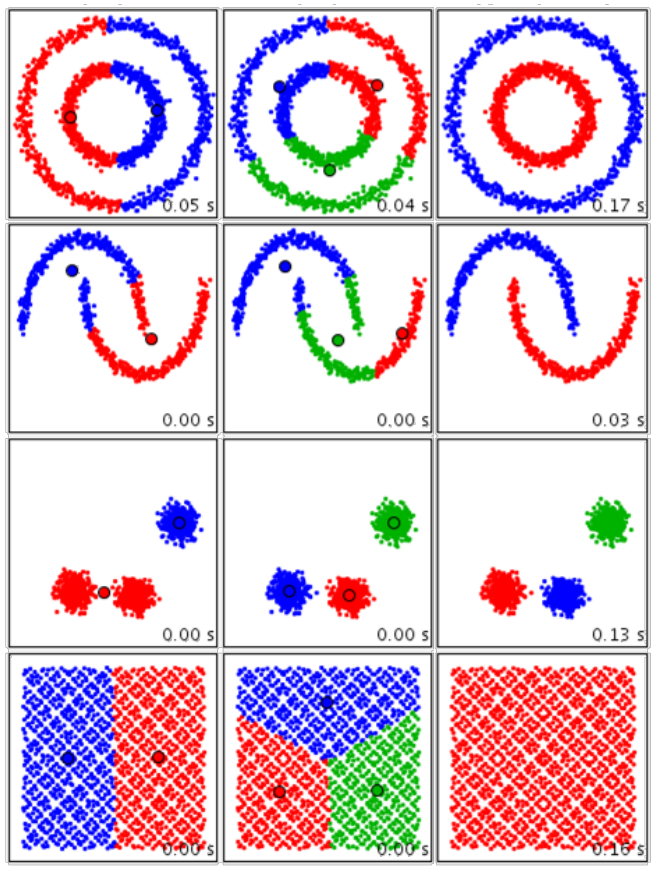
\includegraphics[width=0.6\linewidth]{img/clustering_example}
	\end{center}
\end{minipage}

\subsection{Learnability}
Any target function $f$ over an instance $X$ is learnable given an expressive enough deterministic hypothesis space $\mathcal{H}$, a large enough training set $D$, and stationarity of the distribution $X$, that is instances in $D_{\text{train}}$ and $D_{\text{test}}$ are independently, identically distributed.

Better questions are what size of \textbf{$D_{\text{train}}$} are large enough and given a large enough training set, how well does the \textbf{training error predict generalisability}. These questions are in the domain of \emph{computational learning theory}.

\subsection{Probably Approximate Correct Learning and Vapnik-Chervonenkis Complexity}
Sample complexity bounds using $\abs{\mathcal{H}}$ usually do substantially overestimate, thus the assumption that $\bm{f} \in \mathcal{H}$ is unrealistic.

Measuring Vapnik-Chervonenkis (VC) dimension for infinite $\mathcal{H}$:
$h\in\mathcal{H}$ is \textbf{shattering a set of instances} $S\in X$ \textbf{iif} $h$ can partition $S$ in any way possible.\\
$VC(\mathcal{H}) := \abs{\{S\in X | S \text{ is the largest subset of } X \text{ shattered by any } h\in\mathcal{H}\}}$. $VC(\mathcal{H})$ can be used as an alternative measure of $\abs{\mathcal{H}}$ to compute sample complexity.

\begin{figure}[H]
	\centering
	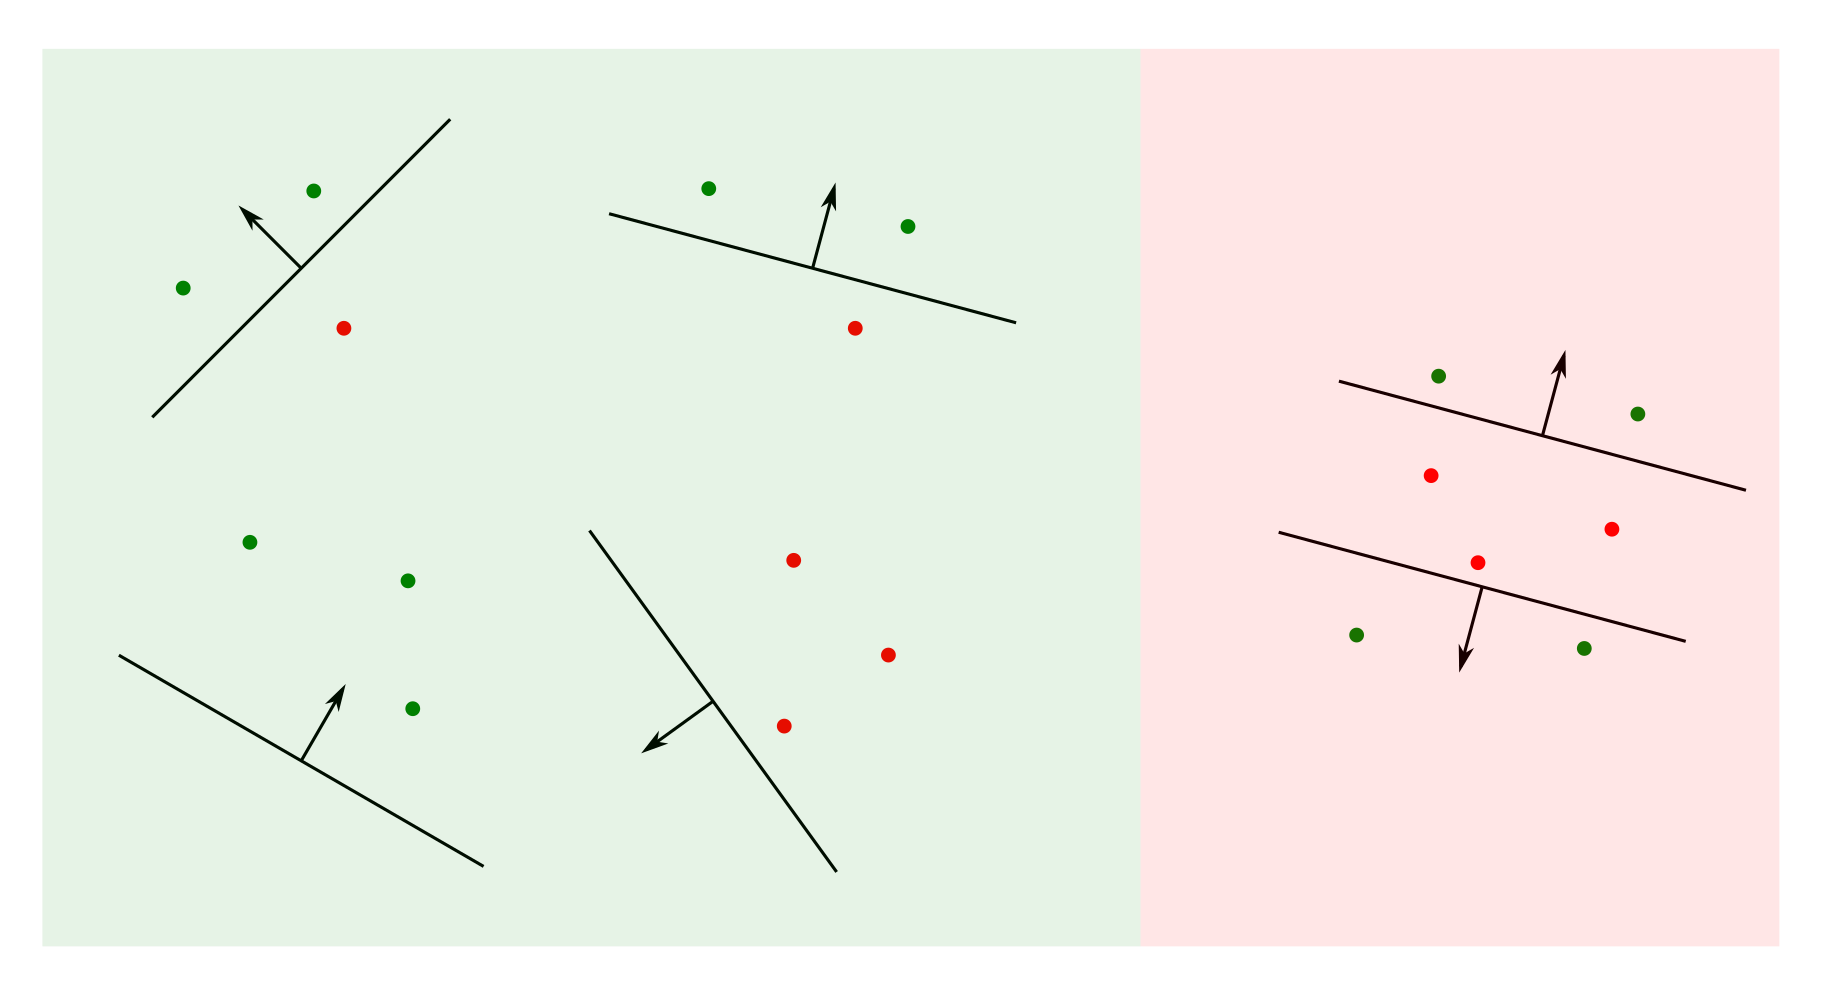
\includegraphics[keepaspectratio,width=0.9\linewidth]{VC_shattering}
	\caption{A two-dimensional linear classifier can shatter three points, $VC(\text{two-dimensional straight lines}=3$ but $\abs{\mathcal{H}} = \infty$}
\end{figure}

\section{Formulating Learning Problems}
\subsection{Designing a Learning Solution}
\begin{center}
	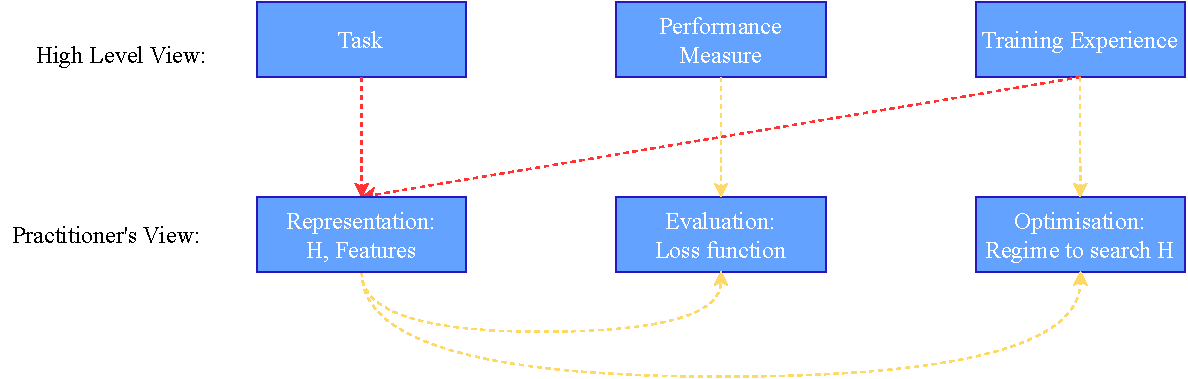
\includegraphics[width=\linewidth,keepaspectratio]{designing_learning_solution.pdf}
\end{center}

Designing a problem that is easiest for the algorithm to solve is the best thing one could do while formulating the problem. The first thing to do while first analysing data is to plot it.

\subsection{Machine Learning Development Process - Exploration and Experimentation}
There is a necessity to have a distinct conceptual approach to model data. Focus on \textbf{systematic experimentation} and \textbf{rigorous evaluation}, even automatised if needed. This is best implemented by a \textbf{pipeline of scripts} similar to the UNIX command line approach. Data exploration and rapid prototyping is key in the beginning of this process.

\begin{center}
	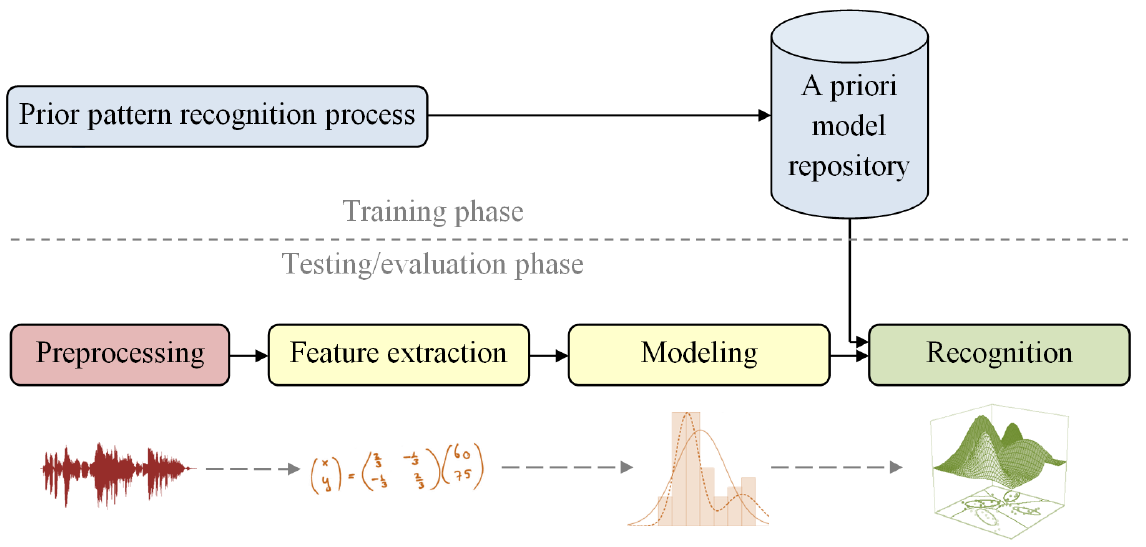
\includegraphics[width=0.6\linewidth]{exploration_evaluation_pipeline}
\end{center}

\section{Machine Learning Guiding Principles}

\subsection{Cost Function J}
Choose $\theta_0, \theta_1$ in such a way that $h(x)$ is close to $y$ for the training examples $(x,y)$. Let a function $J$ \textbf{number the cost of errors made} for the specific set of parameters.

\begin{equation*}
	J_{MSE}(\theta_0, \theta_1) = \frac{1}{2N} \sum_{i=1}^{N} \left(h(x_i, \vec{\theta}) - y_i\right)^2
\end{equation*}

The objective is to minimise $J$ with regards to $\theta_0, \theta_1$

\subsection{Optimisation by Gradient Descent}
Algorithm
\begin{itemize}
	\item Start with a random $\theta_0, \theta_1$
	\item Keep changing $\theta_0, \theta_1$ in a way to reduce $J(\theta_0, \theta_1)$
	\item End at a local minimum
\end{itemize}

\begin{align*}
	\text{\texttt{tmp\_0}} &:= \theta_0 - \alpha \cdot \frac{\partial J}{\partial \theta_0} J(\theta_0,\theta_1)\\
	\text{\texttt{tmp\_1}} &:= \theta_1 - \alpha \cdot \frac{\partial J}{\partial \theta_1} J(\theta_0,\theta_1)\\
	\theta_0 &:= \text{\texttt{tmp\_0}}\\
	\theta_1 &:= \text{\texttt{tmp\_1}}\\
\end{align*}

$\alpha$ is called the learning rate, and is a data-dependent hyper-parameter of the algorithm.

\section{Model Assessment and Selection}

\subsection{Data Handling for Model Evaluation}
Search for methods that help to learn and evaluate algorithms based on \emph{limited data} and help to \emph{deduce the true error} from the training error.

\begin{itemize}[leftmargin=*, labelindent=3cm, labelsep=1cm]
	\item[Model Assessment] \textbf{Evaluate} a model's \textbf{performance}
	\item[Model Selection] \textbf{Select} among competing models the one with the \textbf{proper level of flexibility}
\end{itemize}

\begin{center}
	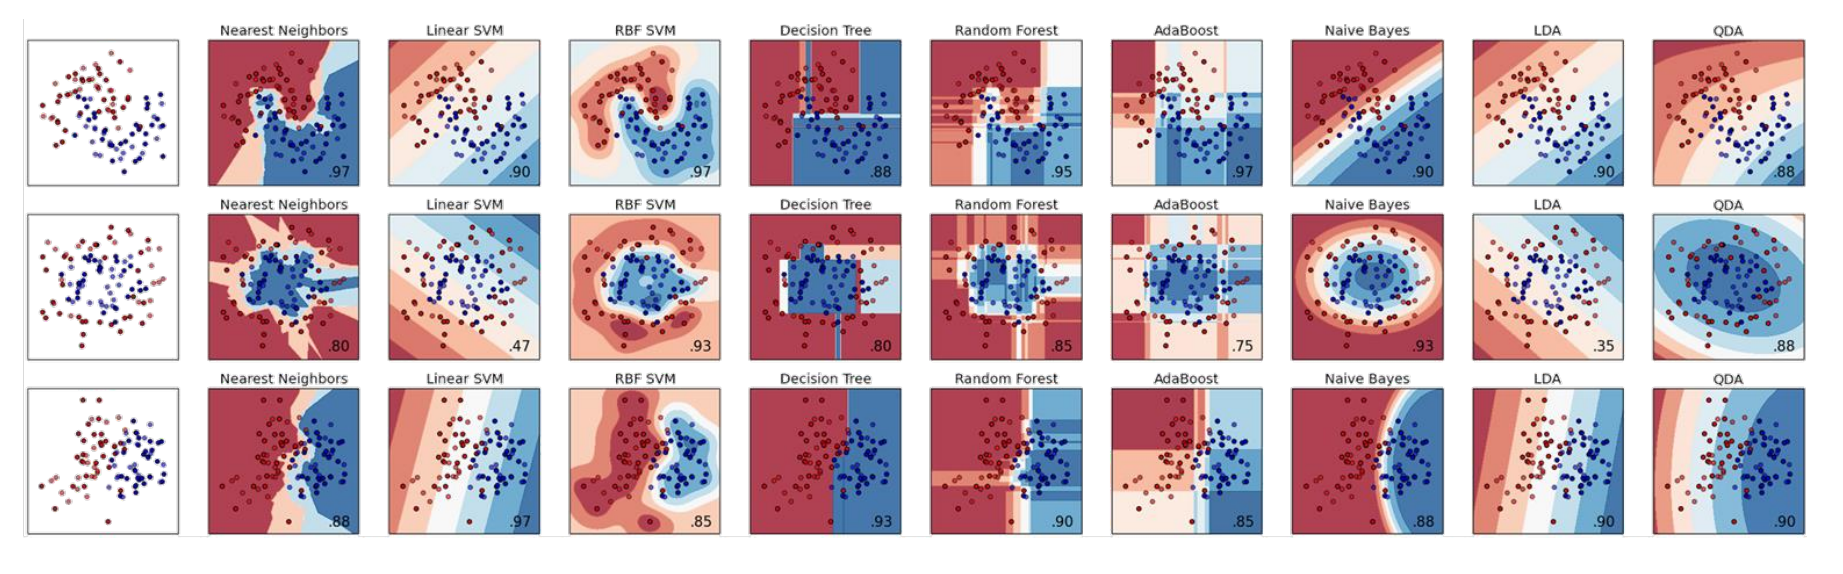
\includegraphics[width=0.9\linewidth]{img/model_flexibility}
\end{center}

\subsection{Optimal Usage of a Small Dataset}
Split into Training, Validation and Test set. Do k-fold Cross Validation on Training and Validation set, final test on Test set. Train k times on $(l - 1)$ folds, validate on the remaining one (until each fold was used for validation once), then average the error.

\subsection{Observable and Unobservable Errors}
True error $E_D$ is the probability that $h$ will misclassify a random instance from the \textbf{complete domain} $\bm{E}$ and is unobservable.

The empirical test error $E_{emp}$ is the proportion of \textbf{sample $S\in D$} misclassified by $h$ is en estimate for the true error and gets better with more error.

\begin{itemize}
	\item Assumption that training and test data are representative of underlying distribution of $D$
	\item $S$ and $h$ are usually not chosen independently, that means that the test error is \textbf{optimistically biased}
	\item The test error usually varies for different $S\in D$, that means it has a higher variance than the true error
\end{itemize}

\subsection{Error Sources}

The chosen hypothesis $\mathcal{H}$ is the \textbf{best hypothesis at a distance of the true function}. Different chosen samples $X$ give \textbf{different information}.

\noindent
Error decomposition:
\begin{equation*}
	E_{MSE} = \underbrace{\text{systematic error}}_{\text{bias}} + \underbrace{\text{dependence on specific sample}}_{\text{variance}}  + \underbrace{\text{random nature of process}}_{\text{irreducible noise or Bayes rate}}
\end{equation*}

\subsection{ROC Curve}
First used in signal detection to show trade-off between \textbf{hit rate} and \textbf{false alarm rate} over noisy channel

\begin{center}
	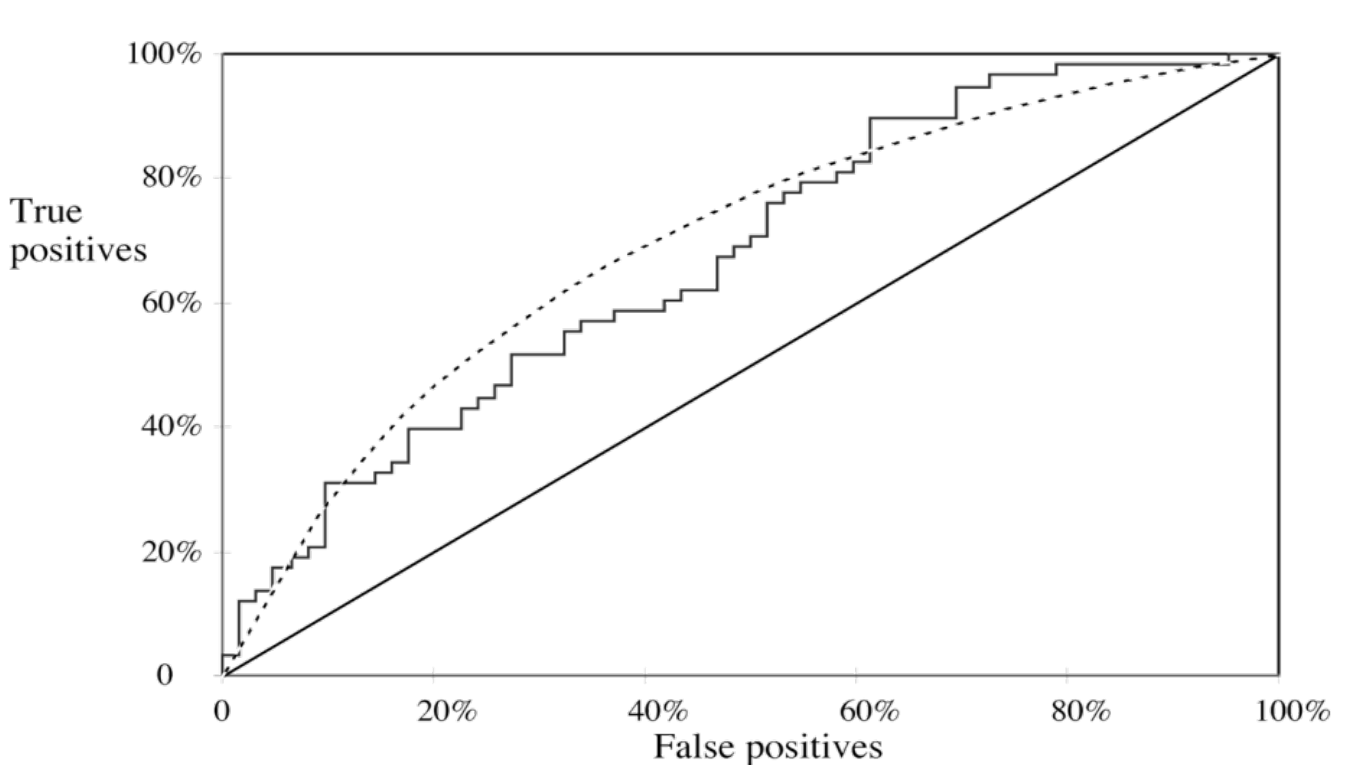
\includegraphics[width=0.7\linewidth]{img/ROC_curve}
\end{center}

\noindent
\textbf{Interpretation}
\begin{itemize}[leftmargin=*, labelindent=3cm, labelsep=1cm]
	\item[Straight Line] Indicates a random process
	\item[Jagged Curve] Created with one set of test data
	\item[Smooth Curve] Created using averages
\end{itemize}

\subsection{Error Measures}
\begin{tabularx}{\linewidth}{lX}
	Mean Square Error & $ E_{MSE} = \frac{1}{F}\sum_{i=1}^{N} (\widehat{y}_i - y_i)^2 $\\
	Root Mean-Squared Error & $E_{RMSE} = \sqrt{\frac{1}{F}\sum_{i=1}^{N} (\widehat{y}_i - y_i)^2 } $\\
	Mean Absolute Error & $ E_{MAE} = \frac{1}{F}\sum_{i=1}^{N} \abs{\widehat{y}_i - y_i}$\\
	(less sensitive to outliers)
\end{tabularx}

\subsection{Evaluating Clustering Methods}
\textbf{Without Labels}:\\
Use the \textbf{silhouette coefficient}, which is a measure for cluster validity or consistency, do a visual inspection of dendrograms and a visual comparison of the dimension reduction o the feature vectors.

\vspace{1em}
\noindent
\textbf{With ground truth available}
Check \textbf{purity}, \textbf{rand index} and \textbf{misclassification rate}.

\subsection{Selection Among Competing Models}
On what basis can one \emph{algorithm be favoured over another} and how probable is it that the chosen method is \emph{truly significantly better}.

\subsection{Maximum Likelihood and Ockham's Razor}
Given competing $h_i \in \mathcal{H}_j$ \textbf{maximum likelihood parameters} can be found by \textbf{calculating the likelihood} $p(X|h_i)$ and \textbf{selecting the best} $\hat{h} = \underset{h_i}{\max} p(X|h_i)$.

The goal is to find a compromise between model complexity and accuracy on the validation data. Ockham's razor, an axiom in machine learning, states that "given two models with the \textbf{same empirical error}, the simpler one should be preferred because \textbf{simplicity is desirable in itself}". The reasoning is that for a simple hypothesis the \textbf{probability of it having unnecessary conditions is reduced}.

\subsection{Determining True Best Classifier}
In practice tenfold cross validation is often good enough and it does not matter which classifier is really better. Otherwise the \textbf{Student's t-test} can be used to compare two samples. Generally, the difference between $\mu_{\mathcal{L}_A}$ and $\mu_{\mathcal{L}_A}$ of the obtained cross-validation error estimates follows a Student's distribution with $m-1$ degrees of freedom.

If the number of features $p$ is large in comparison to the number of instances $N$ use \textbf{boosting} or \textbf{SVM}. If the data set is \emph{severely imbalanced}, \textbf{non-standard loss functions} that take class distribution in account or \textbf{Bayesian methods} and appropriate prior probabilities should be considered.

\section{Support Vector Machines}

Each observation is a vector of values ($p$-dimensional) for which the SVM \textbf{constructs a hyperplane} to separate class members. There are different support vectors for different tasks
\begin{enumerate}
	\item Maximal margin \textbf{hyperplane} classifier, for linearly separable data
	\item Support vector \textbf{classifier}, for almost linearly separable data
	\item Support vector \textbf{machine}, for non-linearly separable data
\end{enumerate}

\subsection{Maximal Margin Classifier}
\begin{minipage}{0.6\linewidth}
	Chooses the hyperplane maximising the distance from the hyperplane to the closest training point, denoted the support vectors, and can be represented as a linear combination of only a few training points.
\end{minipage}
\begin{minipage}{0.4\linewidth}
	\centering
	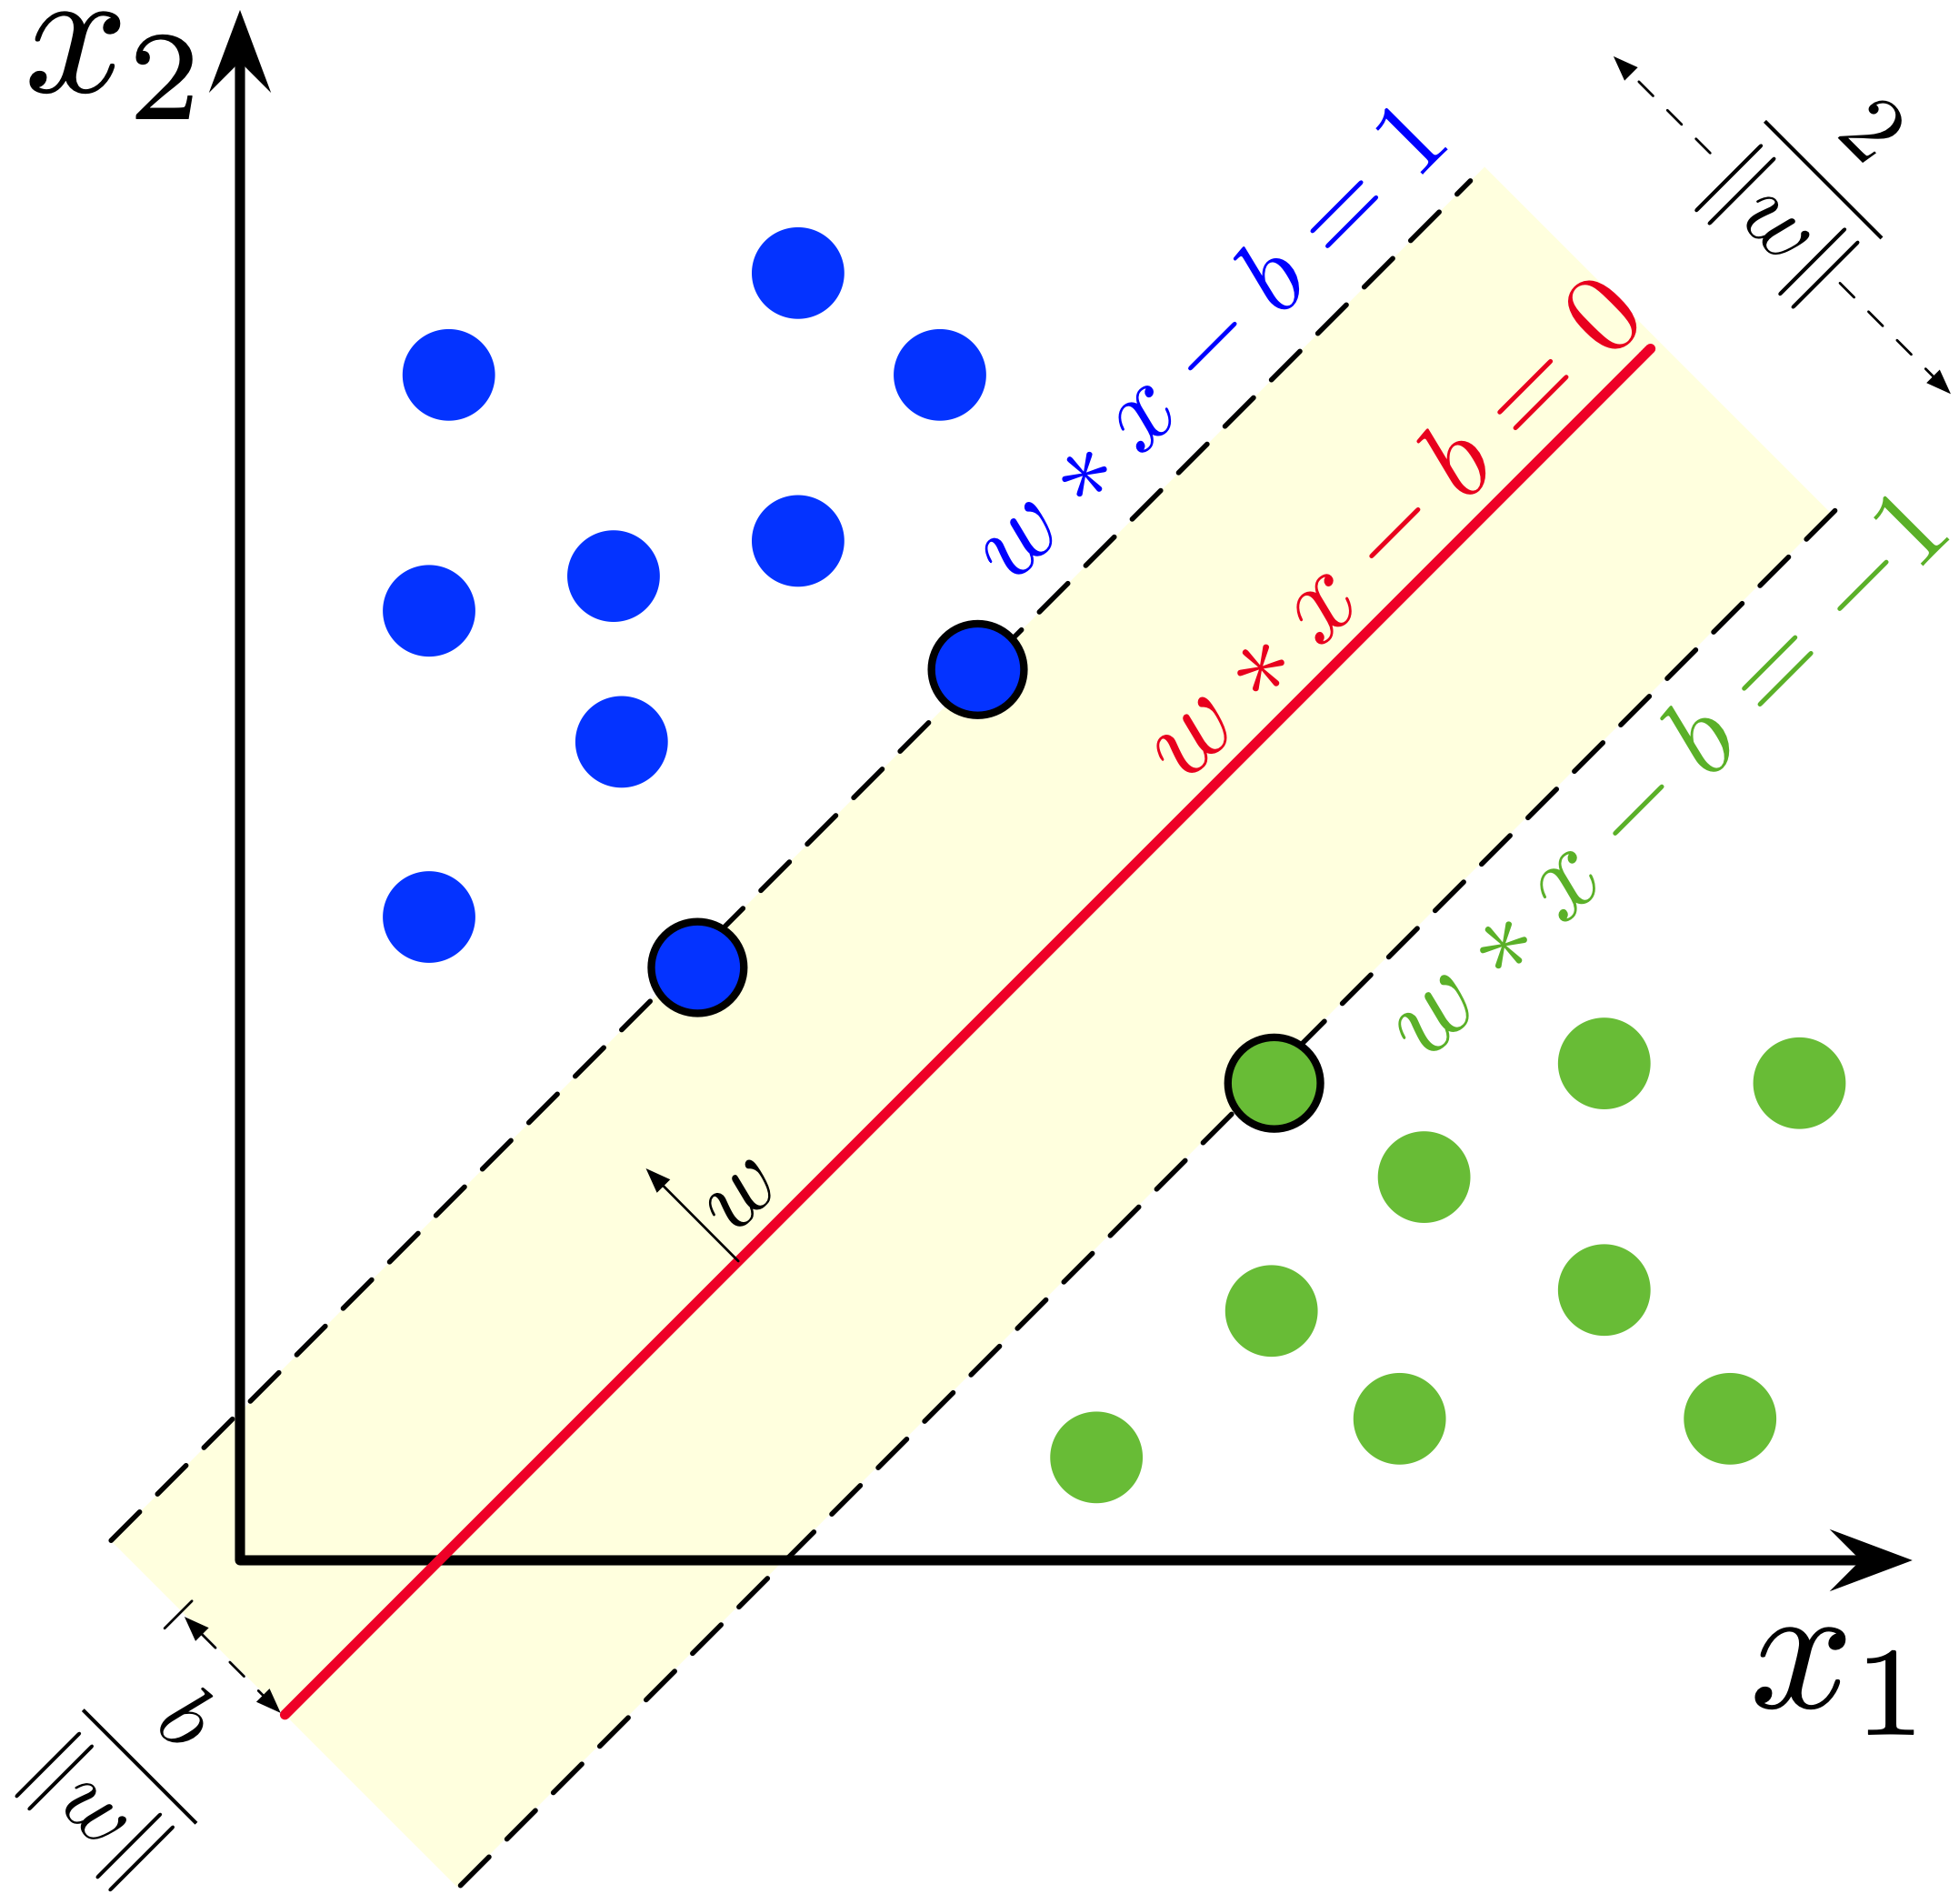
\includegraphics[keepaspectratio,width=0.8\linewidth]{img/maximum_margin_classifier.png}
\end{minipage}

\begin{definition}
	Definition of a hyperplane
	\begin{equation*}
		\{ \vec{x}: \beta_0 + \beta_1 x_1 + \beta_2 x_2 + \dots + \beta_p x_p = 0 \}
	\end{equation*}
\end{definition}
Separating hyperrplanes for classes encoded $\pm 1$
\begin{align*}
	\beta_0 + \beta_1 x_{i1} + \beta_2 x_{i2} + \dots + \beta_p x_{ip} &> 0 \qquad \text{ if } y_i = 1\\
	\beta_0 + \beta_1 x_{i1} + \beta_2 x_{i2} + \dots + \beta_p x_{ip} &< 0 \qquad \text{ if } y_i = -1\\
	\intertext{Equivalently}
	y_i\cdot (\beta_0 + \beta_1 x_{i1} + \beta_2 x_{i2} + \dots + \beta_p x_{ip}) &> 0
\end{align*}
Evaluating the hyperplane formula for a point $x$ gives its distance to the hyperplane, if $\bm{\beta}$ is a normal vector.

\subsection{Formulation of Optimisation Problem}
Intuitive Optimisation
\begin{itemize}[noitemsep]
	\item $\underset{\beta_0,\beta_1,\dots,\beta_p}{\text{maximise}} M$
	\begin{itemize}
		\item subject to $\sum_{j=1}^{p}\beta_j^2 = 1$
		\item and $y_i\cdot (\beta_0 + \beta_1 x_{i1} + \beta_2 x_{i2} + \dots + \beta_p x_{ip}) \geq M\qquad\forall i = 1..N$
	\end{itemize}
\end{itemize}
This can be reformulated using {\color{DodgerBlue2} Lagrange multipliers}
\begin{itemize}[noitemsep]
	\item Find $L_D = \sum_{i=1}^{N} \alpha_i - \frac{1}{2} \sum_{i=1}^{N}\left( \sum_{k=1}^{N} \alpha_i \alpha_k \bm{x}_i^T \bm{x}_k \right) $
		\begin{itemize}
		\item subject to $ \alpha_i \geq 0 $ and $\sum_{i=1}^{N} \alpha_i y_i = 0$
		\item Once the alphas are computed $\beta = \sum_{i=1}^{N} \alpha_i y_i \bm{x}_i$
	\end{itemize}
\end{itemize}

\subsection{Support Vector Classifier}
Based on the assumption that the data is not perfectly linearly separable any more, the idea is to introduce soft margins that allow for \emph{some} misclassifications. The number of misclassifications is controlled by a {\color{DodgerBlue2} penalty factor} $C$.

\begin{center}
	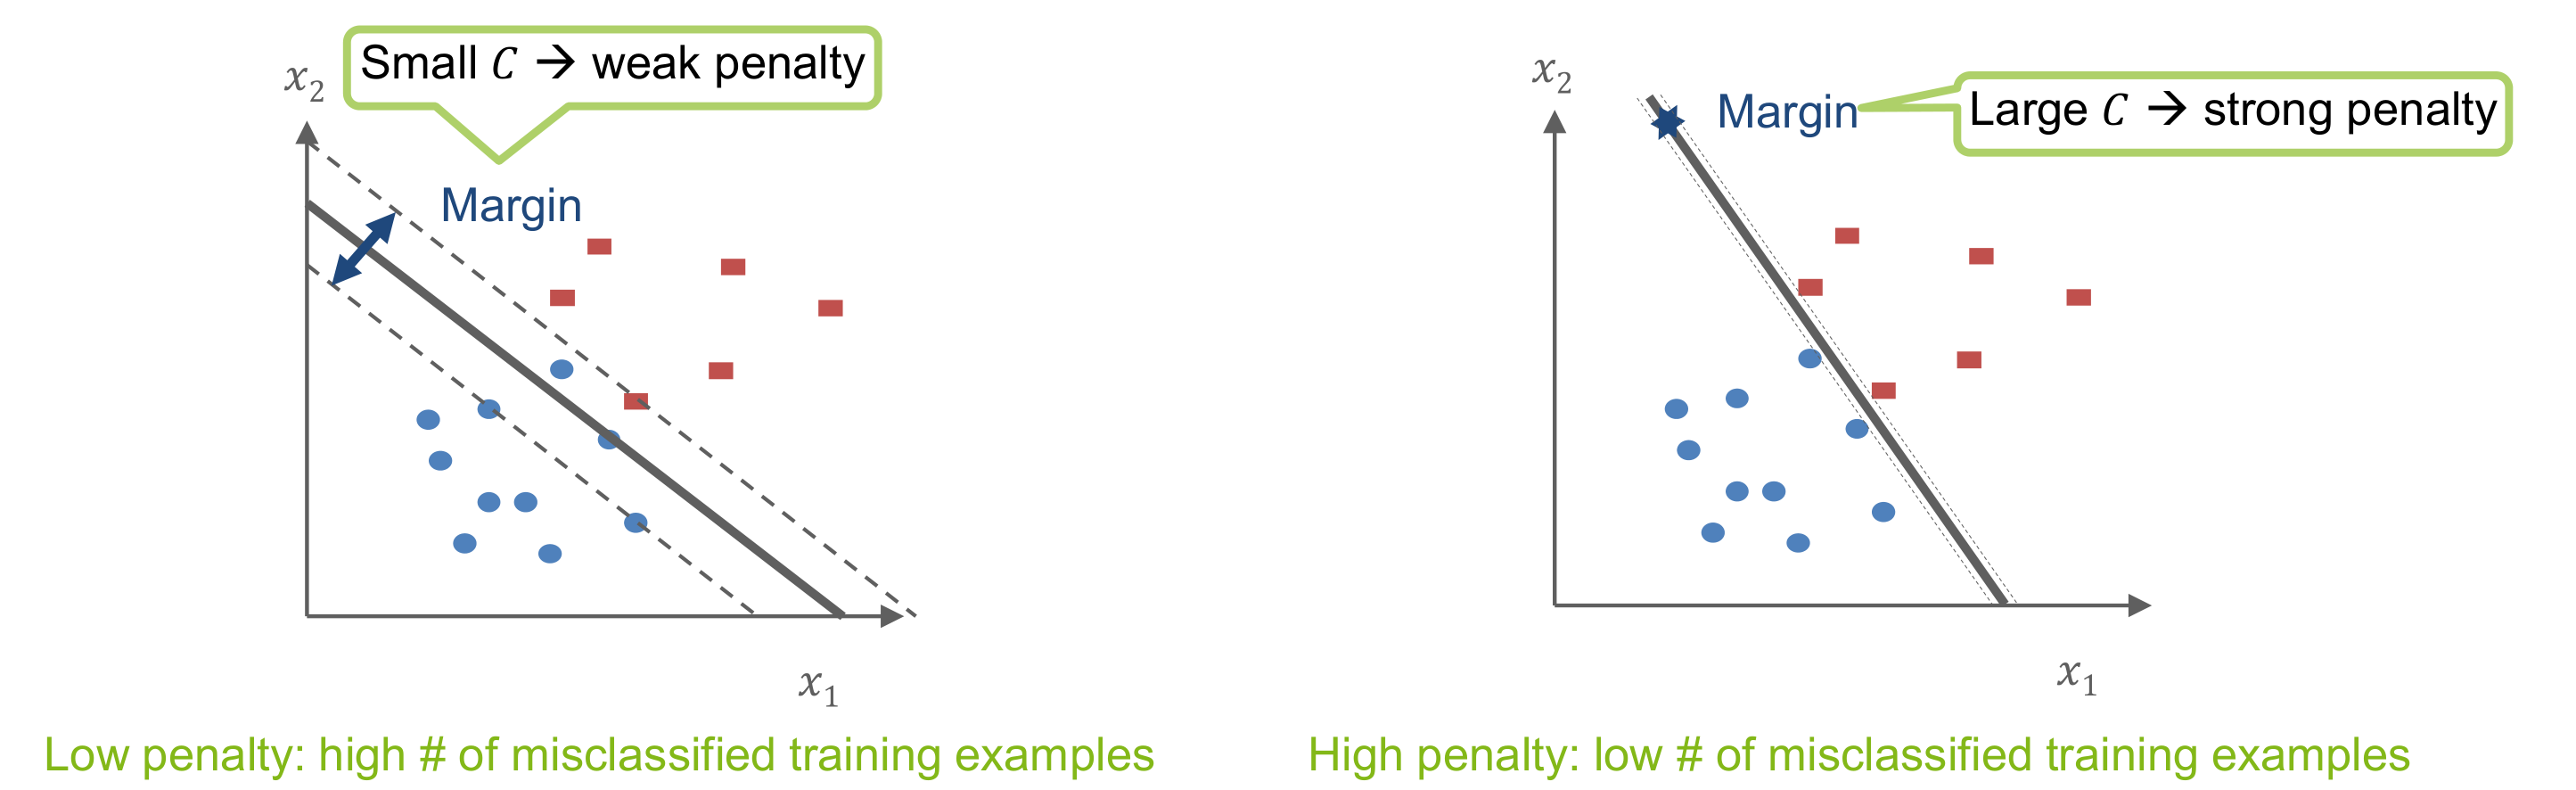
\includegraphics[width=0.7\linewidth]{img/support_vector_classifier}
\end{center}

\subsubsection{Support Vector Classifier Optimisation}
\begin{minipage}{0.6\linewidth}
Intuitive Optimisation
\begin{itemize}[noitemsep,nosep]
	\item $\underset{\beta_0,\beta_1,\dots,\beta_p}{\text{maximise}} M$
	\begin{itemize}
		\item subject to $\sum_{j=1}^{p}\beta_j^2 = 1$
		\item and $y_i\cdot (\beta_0 + \beta_1 x_{i1} + \beta_2 x_{i2} + \dots + \beta_p x_{ip}) \geq M(1 - \xi_i)   \qquad\forall i = 1..N$
		\item $\xi_i \geq 0, \sum_{i=1}^{N}\xi_i \leq \tilde{C}$
		\item where $\xi_i$ is a slack variable to allow instance $i$ to lie on the wrong side of the margin
		\item $\tilde{C}$ is the total budget for misclassifications
	\end{itemize}
\end{itemize}
Equivalent technical optimisation, so called "dual form"
\begin{itemize}[noitemsep,nosep]
	\item maximise\\
	$L_D = \sum_{i=1}^{N} \alpha_i - \frac{1}{2} \sum_{i=1}^{N}\sum_{k=1}^{N} \alpha_i \alpha_k y_i y_k x_i^T x_k$
	\begin{itemize}
		\item subject to $0 \leq \alpha_i \leq C$ and $\sum_{i=1}^{N}\alpha_i y_i = 0$
		\item $\beta = \sum_{i=1}^{N} \alpha_i y_i x_i$ is minimised
	\end{itemize}
\end{itemize}
\end{minipage}
\begin{minipage}[t]{0.4\linewidth}
		\centering
		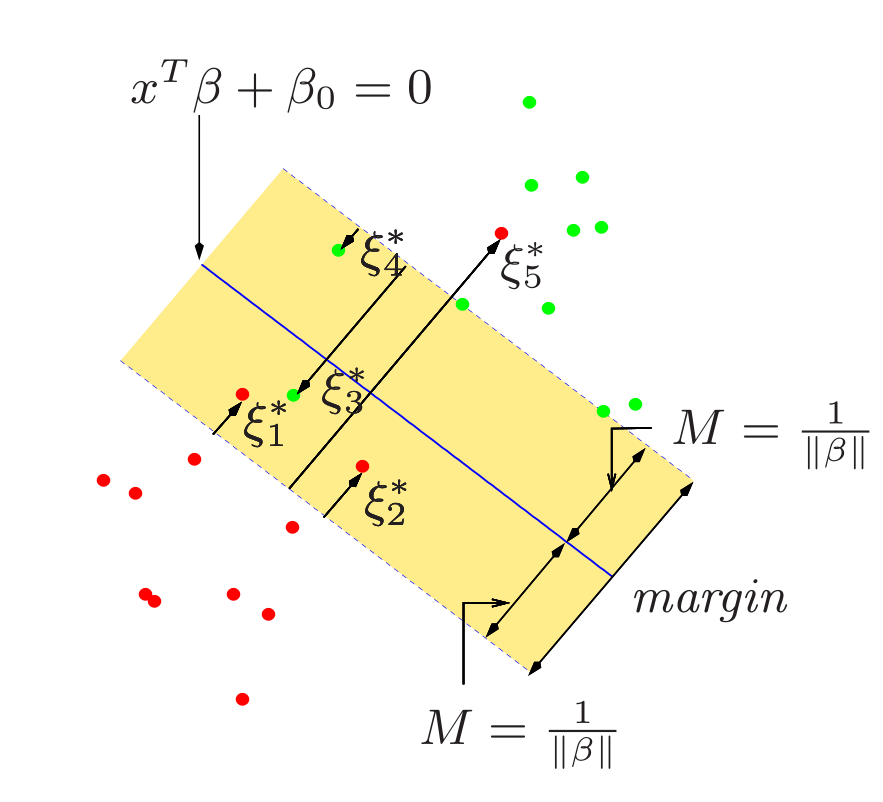
\includegraphics[width=0.8\linewidth]{img/support_vector_classifier_penalty}
\end{minipage}

\subsection{Support Vector Machines}
A possible solution for linearly completely non-separable data is to map the data into a higher-dimensional space. In this space a separating hyperplane may be defined. 

\subsubsection{Variable Transformation}
The same idea applies, transform a non-linearly separable input function in $\R^n$ to $\R^{n+k}, k\geq 1$ where it may be linearly separable.

\begin{center}
	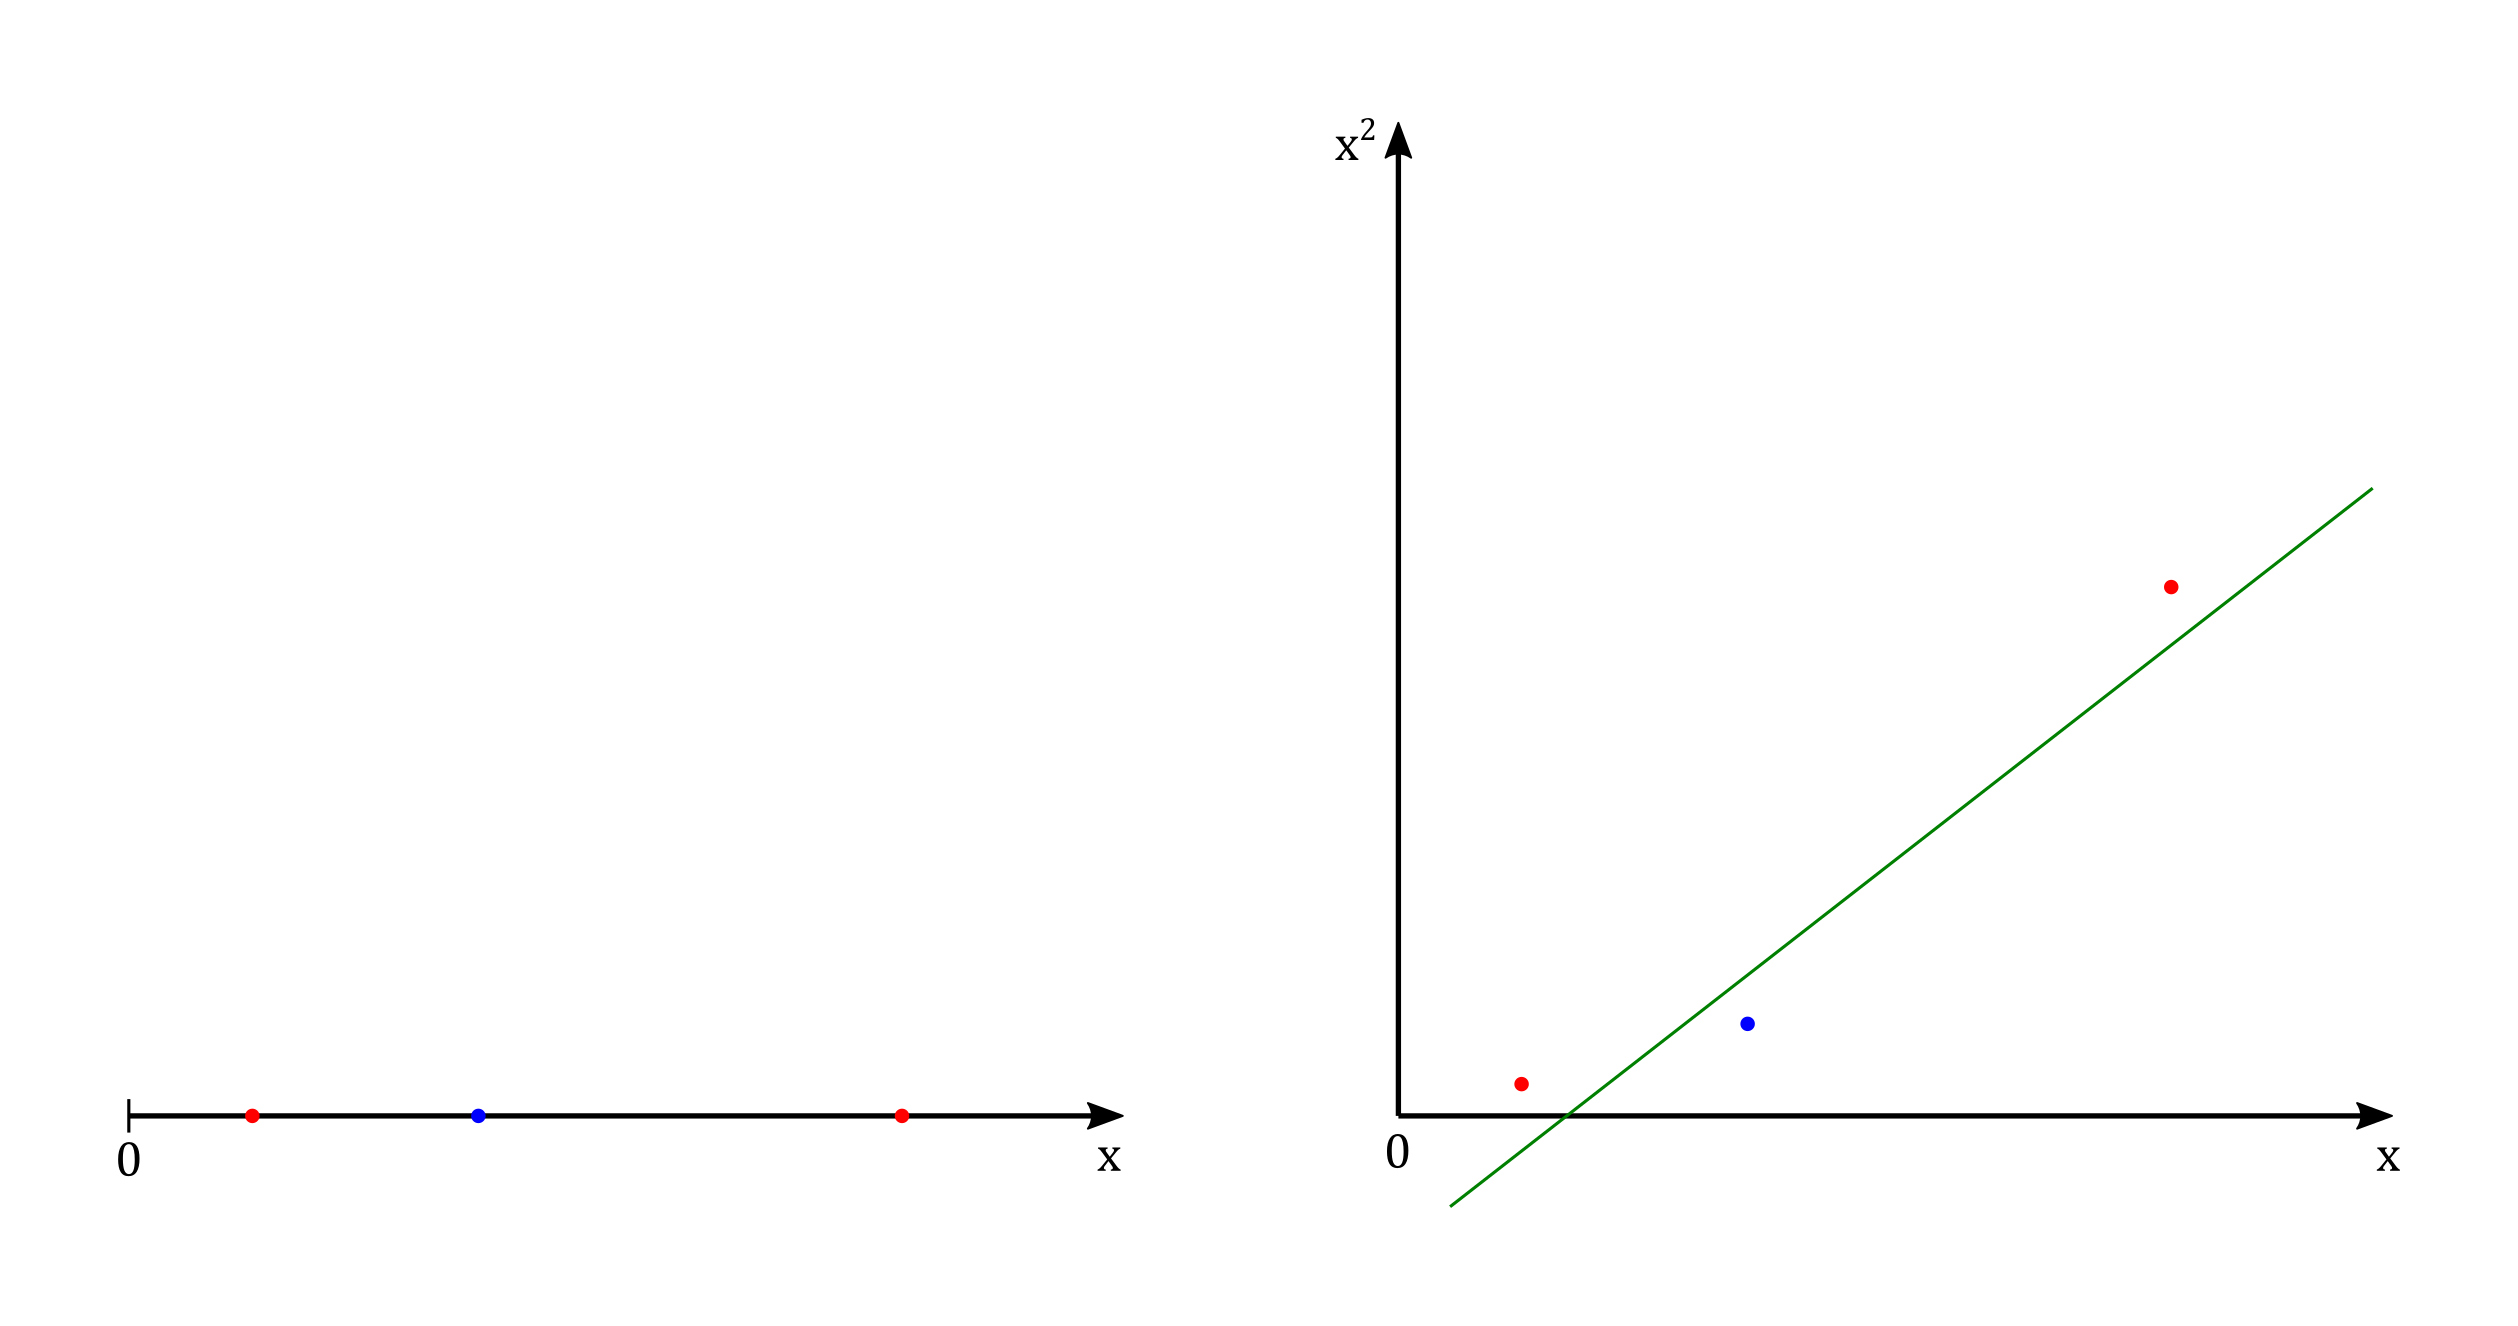
\includegraphics[keepaspectratio,width=0.6\linewidth]{variable_transformation.png}
\end{center}

The power of feature space transformation lies in the fact, that with an appropriately chosen feature space of sufficient dimensionality any consistent training set can be made separable.
\begin{equation*}
	\left\langle \begin{pmatrix}x_i\\x_i^2\end{pmatrix} \cdot\begin{pmatrix}x_{i'}\\x_{i'}^2\end{pmatrix} \right\rangle = x_i x_{i' } + x_i^2 x_{i' }^2 := K(x_i,x_{i'})
\end{equation*}
$K$ is known as a \textbf{kernel} function. It can be used to efficiently compute feature space transformations. Instead of calculating the inner product, the kernel $K(\cdot,\cdot)$ gets calculated. As soon as some $K$ is used, the resulting SVC becomes a SVM.

The following Kernels are common
\begin{itemize}[noitemsep]
	\item {\color{DodgerBlue2} Identity (inner product)}
	\begin{equation*}
		K(x_i,x_{i'}) = \sum_{j=1}^{p} x_{ij}x_{i'j}
	\end{equation*}
	this yields the standard support vector classifier
	\item {\color{DodgerBlue2} Polynomial of degree $d$}
	\begin{equation*}
		K(x_i,x_{i'}) = \left(1 + \sum_{j=1}^{p} x_{ij}x_{i'j}\right)^d
	\end{equation*}
	the polynomial kernel of degree $d = 1$ is just the identity kernel
	\item {\color{DodgerBlue2} Radial basis or Gaussian}
	\begin{equation*}
		K(x_i,x_{i'}) = e^{\left( -\gamma \sum_{j=1}^{p}(x_{ij} - x_{i'j})^2 \right)}
	\end{equation*}
	the Gaussian kernel computes a very local neighbourhood, with $\gamma$ being the hyper-parameter controlling the width of that neighbourhood. A low $\gamma$ yields a great width. The feature space spanned by the Gaussian kernel is implicit and infinite-dimensional.
\end{itemize}

\subsection{Multiclass Classification With Support Vector Machine}
With one versus rest or all classification, the binary classifier SVM can be adapted to choose between multiple classes.
\begin{center}
	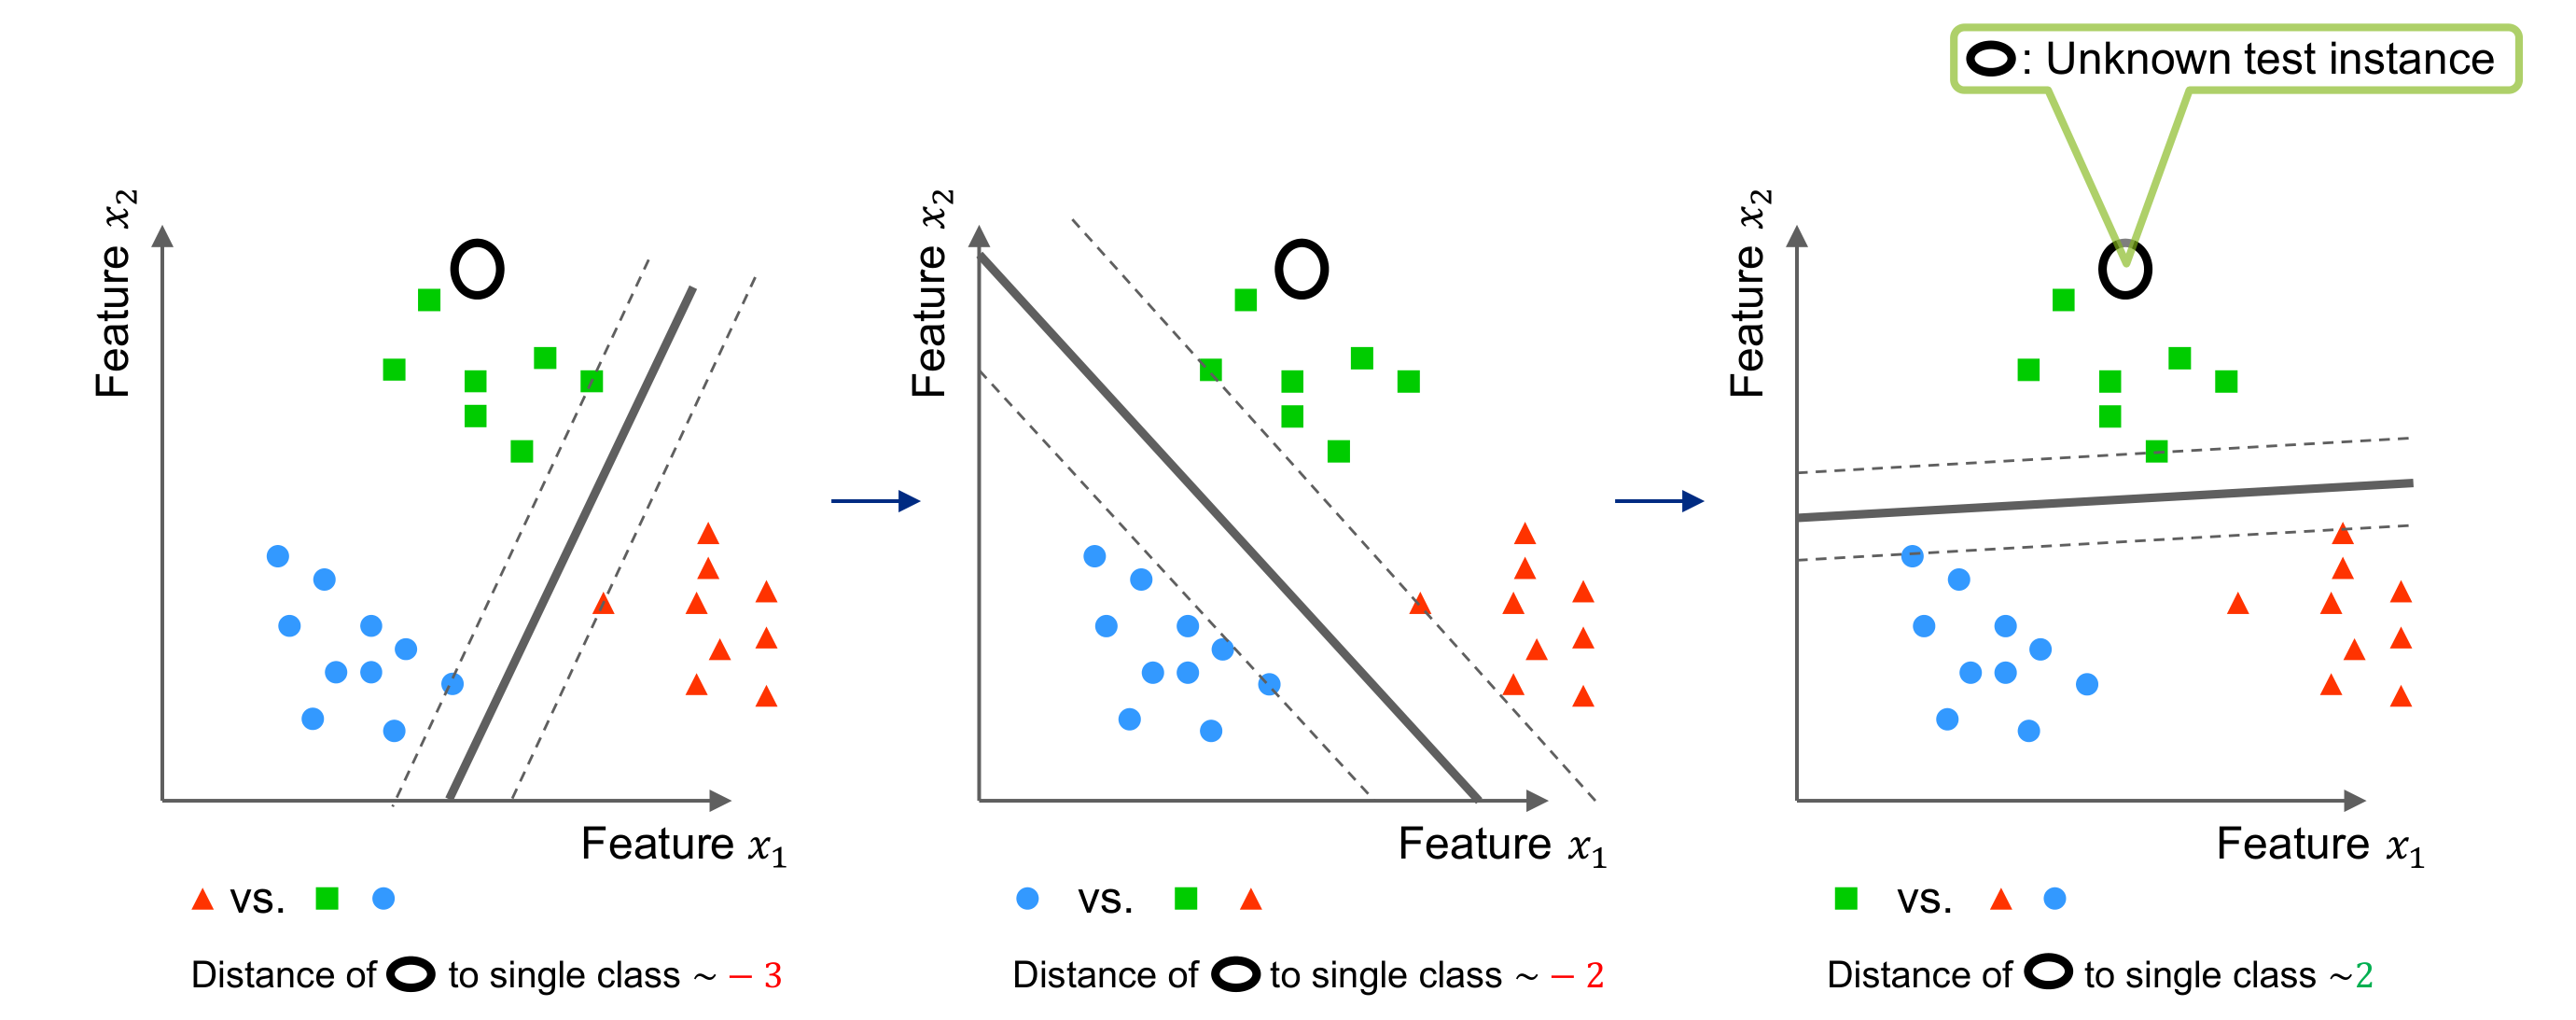
\includegraphics[width=0.8\linewidth]{img/support_vector_machine_multiclass}
\end{center}
Assume $k$ classes, learn all $\frac{k(k-1)}{2}$ pairwise comparisons and classify unknown instances by majority vote among all pairwise comparisons.

\section{Ensemble Methods}
The goal of ensembles is to increase performance by \textbf{combining multiple complementary classifiers}. The intuition behind it is to build different experts and let them decide by vote. This is {\color{Green3} very effective in practice} and has {\color{Green3}good theoretical guarantees}, but while being {\color{Green3} easy to implement} the result {\color{Firebrick3} lacks in transparency}, {\color{Firebrick3}interpretability} and a {\color{Firebrick3} compact representation}.

The formal problem description is: Given $T$ binary classification hypotheses $(h_1,\dots, h_T)$, find a combined classifier with better performance of the form
\begin{equation*}
	\hat{h}(x) = \text{sign}\left( \sum_{t=1}^{T} \alpha_t h_t (x) \right)
\end{equation*}
For regression the average is used.

Ensembles work because they average the error, in statistical terms the bias remains equal but the variance is reduced.

\subsection{AdaBoost}
\subsubsection{Boosting}
The general idea is to boost the performance of weak learners iteratively by making misclassified examples more important and then combining hypotheses. This way, each stage additively corrects shortcomings of previous stages by reweighing and majority voting on the result. The \textbf{Ada}ptive \textbf{Boost}ing algorithm works by
\begin{minted}[escapeinside=||,mathescape=true,fontsize=\small]{python}
initialize weights: |$w_i := \frac{1}{N}$|
for |$ t:=1..T $|
	|$ h_t $| := train decision stump on the |$ x_i $|, weighted by the |$ w_i $|
	|$ \varepsilon_t $| := |$ \frac{\sum_{i=1}^{N} w_i \cdot I(y_i\neq h_t(x_i) }{\sum_{i=1}^{N} w_i} $| # compute error, $ I() $ is the identity function
	|$ \alpha_t $| := |$ \log\left(\frac{1-\varepsilon_t}{\varepsilon_t} \right) $| # compute influence of weak learner
	|$ w_i $| := |$ w_i\cdot e^{\alpha_t\cdot I(y_i \neq h_t(x))} $| # increase weight by exp(Influence) in case of error
return |$ \hat{h} $| := |$ \text{sign}\left(\sum_{t=1}^T \alpha_t\cdot h_t(x)\right) $| # majority vote
\end{minted}



\end{document}
